\subsection{Practical algorithm}
The augmented graph may contain a lot of unnecessary information.
For example, the same efficient path $uv$ can be repeated many times in the form $\pp{u,1}\pp{v,0}$, $\pp{u,2}\pp{v,1}$ and so on.
If there are not too many efficient paths, we can obtain considerable improvements both in query time and in data storage.

The idea is to construct an augmented graph without duplicated information.
The nodes are, as before, pairs $\pp{v,b}$, but an edge $(\pp{v,b},\pp{v',b'})$ is placed only if some efficient path uses it.
In other words, if we let $\calP_{s,t}^E$ be the set of all efficient paths from $s$ to $t$, we take every $P\in \calP_{s,t}^E$ with cost $b\leq B$ and trace it in the augmented graph starting at $\pp{s,b}$ and ending at $\pp{t,0}$.

\begin{definition}
The pruned augmented graph is defined by $\Gp^B=(\Vp^B,\Ep^B)$, where
\begin{align*}
\Vp^B &:=\{\pp{v,b}: v\in V, b=0,1,\ldots,B\},\\
\Ep^B &:=\{\pp{v,b}\pp{v',b'} : \exists s,t\in V, P\in\calP^E_{s,t}, c(P)\leq B, \\
&\qquad vv'\in P, b=c(P[v,t]), b'=c(P[v',t])  \}.
\end{align*}
In $\Gp^B$ all the lengths are preserved.
\end{definition}
Note that in $\Gp^B$ there are no sink nodes, hence it has at least $n$ nodes and $nB$ arcs fewer compared to $G^B$.

\subsubsection{HD of the pruned augmented graph}

A shortest path in $\Gp$ does not necessarily project to an efficient path, even if the path ends in a node of the form $\pp{t,0}$.
On the other hand, if $P$ projects to an efficient path, then necessarily $P$ is shortest. 
To bound the HD, the correct system to study is
\[
\tilde\calP^B:=\{P: P\text{ ends in a node }\pp{t,0}, \bar P\in \PE, c(\bar P)\leq B \}.
\]
The following result shows how the HD of this system relates to that of $\PE$.
We omit the proof since it is identical as the one in Proposition~\ref{prop:HDaugmented}.
\begin{proposition}
The HD of $\tilde\calP^B$ is $Bh_c$, where $h_c$ is the HD of $\PE$.
\end{proposition}

We use techniques described by \cite{hubimplem} together with an approach tailored for augmented graphs.
The main idea is to use contraction hierarchies first, then define the forward hub of a node as the nodes visited during a contraction-based forward search.
The backward hub is defined analogously.
These are valid hubs, since the highest rank node in a path is guaranteed to be in both hubs.

The most important parameter in CH is the rank; results vary greatly from one choice of ranks to another.
We obtain a rank in $G$ by running a greedy shortest-path cover, defined as follows.
Start with a cover $C=\varnothing$ and compute the set of all shortest paths $\calP$.
Take a node $v\notin C$ hitting most paths in $\calP$, then remove all those paths from $\calP$, add $v$ to $C$ and iterate.
The rank is defined as $n$ for the first node added to $C$, $n-1$ for the second and so on.

We work with the pruned augmented graph, i.e.\ $\tilde G_B$, which takes some time to compute, but yields considerably better hubs. 
Recall that in $\tilde G_B$ there are no sink-nodes nor ``replicated information'', since efficient paths are stored just once.
Given a rank for nodes in $G$, we contract $\tilde G_B$ as follows.
Say that $V$ is ordered according to the rank, so node $1$ is the least important and $n$ the most important.
In $\tilde G_B$, for $b=B,\ldots,0$, we contract the nodes $(1,b)$ first, then the nodes $(2,b)$ and so on till the nodes $(n,b)$ are the last to contract. 

To obtain better hubs we prune the results obtained by contraction-based searches.
If $w$ is in the forward search of $v$ with distance $d$, it might be that $\dist(v,w)<d$, this occurs because the search goes only to higher rank nodes and the discovered path is missing some node.
When $\dist(v,w)<d$, we can safely remove $w$ from the hub of $v$, since the highest ranked node in a shortest path will have the correct distance.
We describe now the process in the following steps.

\begin{enumerate}
\item Compute the shortest paths in $G$ and obtain a cover $C$
\item Compute the pruned augmented graph $\tilde G_B$
\item Contract $\tilde G_B$ using the rank given by $C$
\item Create hubs $\Lf(v),\Lb(v)$ using CH
\item Prune the hubs by running HL queries between $v$ and nodes in $\Lf(v)$. 
Run a similar process for $\Lb(v)$.
\end{enumerate}
Note that in the last step we bootstrap HL to improve it.
This works because the fact that some nodes have incorrect distance labels does not impact the correctness of a HL query; a node minimizing the distance is returned and such node must have a correct label.

\subsection{Experiments}

All the experiments were run on a 64-bit desktop computer, Intel Core i7-6700, 3.40GHz,  with 16GB RAM and operative system Ubuntu 16.04.
The entire code is in Python 2.7, the main library we use is Networkx, which implements graph representation and Dijkstra's algorithm.
To compute the SP cover we follow the exhibition in \cite{hubimplem}.

We evaluated the performance of our algorithms with real-world test networks: a small San Francisco network with 2643 nodes and 6588 edges for which real-world travel-time data was available as a Gaussian mixture model \cite{sf_data}, and a second (relatively larger) Luxembourg network with 30647 nodes and 71655 edges for which travel-time distributions were synthesized from road speed limits \cite{niknami2016tractable}, as real-world data was unavailable.
Additionally, we tested on the subgraph corresponding to Luxembourg City with 4026 nodes and 9282 edges.

The first experiment was on San Francisco.
We used the following cost structure.
The 10\% edges with the highest variance are assigned cost 1, the rest cost 0.
On Table~\ref{tab:sf_results} we present the results for different maximum budgets $B$.
The column for $B=0$ represents the original graph (without augmentation).
The query times are measured as the average of 1000 random $s,t$ pairs, were the task is to recover $\dist(s,t|b)$ for every $b=0,1,\ldots,B$, i.e., the entire efficient frontier.

\begin{table}\caption{Results for San Francisco}\label{tab:sf_results}
\begin{center}
\begin{tabular}{ | l | p{1cm} | p{1cm} | p{1cm} | p{1.2cm} | p{1.2cm} | }
\hline
	B & Preproc [m] & Avg F Size & Avg B Size & Query Dij [ms] & Query HL [ms] \\ \hline \hline
	0 & 1 & 23 & 22 & 10.71 & 0.005 \\ \hline
	5 & 5 & 17 & 28 & 74.71 & 0.02 \\ \hline
	10 & 13 & 17 & 28 & 183.18 & 0.03 \\ \hline
	15 & 14 & 17 & 28 & 250 & 0.03 \\ \hline
	20 & 21 & 17 & 28 & 489.74 & 0.04 \\ \hline
	25 & 22 & 17 & 28 & 467.84 & 0.04 \\ \hline
	30 & 37 & 17 & 28 & 648.17 & 0.04 \\ \hline
\end{tabular}
\end{center}
\end{table}
 
\begin{table}\caption{Results for Luxembourg City}\label{tab:lu4k_results}
\begin{center}
\begin{tabular}{ | l | p{1cm} | p{1cm} | p{1cm} | p{1.2cm} | p{1.2cm} |}
\hline
	B & Preproc  [m] & Avg F Size & Avg B Size & Query Dij [ms] & Query HL [ms] \\ \hline \hline
	0 & 6 & 18 & 18 & 16.35 & 0.004 \\ \hline
	5 & 23 & 14& 19 & 151.91 & 0.019 \\ \hline
	10 & 36 & 14 & 19 & 305.33 & 0.021 \\ \hline
	15 & 51 & 14& 19 & 490.75 & 0.024 \\ \hline
	20 & 69 & 14 & 19 & 808.90 & 0.030 \\ \hline
	25 & 89 & 14 & 19 & 1016.71 & 0.034 \\ \hline
	30 & 101 & 14& 19 & 1144.07 & 0.032 \\ \hline
\end{tabular}
\end{center}
\end{table}

\begin{figure}\caption{Luxembourg City with different clusters}\label{fig:clusters_lu}
\hfill
\begin{tikzpicture}[trim axis left]
\begin{axis}[
	scale only axis,
	height=3cm,
	width=3.9cm,
	xtick distance=300,
	ytick distance=1,	
	xmin = 10, xmax =1000,
	xlabel={Number of clusters},
	ylabel={},
	every axis plot/.append style={thick}]
\addplot[mark size=0.3,draw=black, mark=square*] table {tab_avg_lu.dat};
\addplot[mark size=0.3,draw=red, mark=triangle*] table {tab_max_lu.dat};
\addplot[mark size=0.3,draw=blue, mark=diamond*] table {tab_shorts_lu.dat};

\legend{Avg hub size, Max hub size,\# shortcuts}
\end{axis}
\end{tikzpicture}

\end{figure}

\begin{figure}\caption{San Francisco with different clusters}\label{fig:clusters_sf}
\hfill
\begin{tikzpicture}[trim axis left]
\begin{axis}[
	scale only axis,
	height=3cm,
	width=3.9cm,
	xtick distance=300,
	ytick distance=1,	
	xmin = 10, xmax =1000,
	xlabel={Number of clusters},
	ylabel={},
	every axis plot/.append style={thick}]
\addplot[mark size=0.3,draw=black, mark=square*] table {tab_avg_sf.dat};
\addplot[mark size=0.3,draw=red, mark=triangle*] table {tab_max_sf.dat};
\addplot[mark size=0.3,draw=blue, mark=diamond*] table {tab_shorts_sf.dat};

\legend{Avg hub size, Max hub size,\# shortcuts}
\end{axis}
\end{tikzpicture}

\end{figure}


\begin{figure}\caption{Significance in Luxembourg City}\label{fig:map_LU} 
\begin{center}
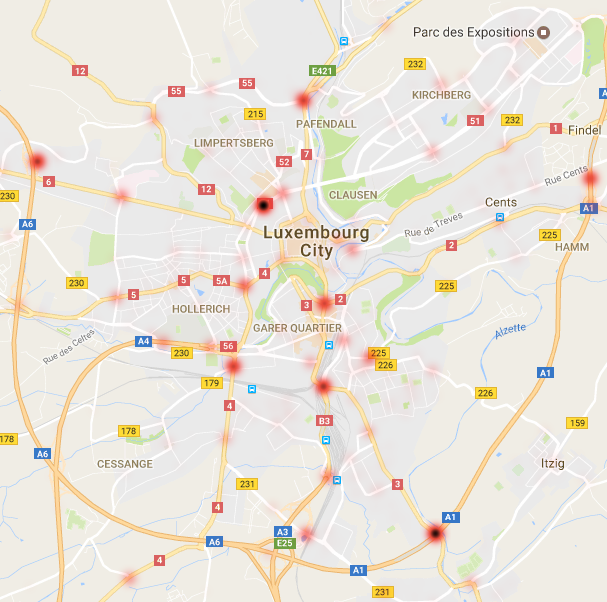
\includegraphics[scale=0.37]{TexImg/map_LU_sig.png}
\end{center}
\end{figure}

\begin{figure} \caption{Size of backward hubs, $B=25$}\label{fig:SF_bwd_size}
\begin{center}
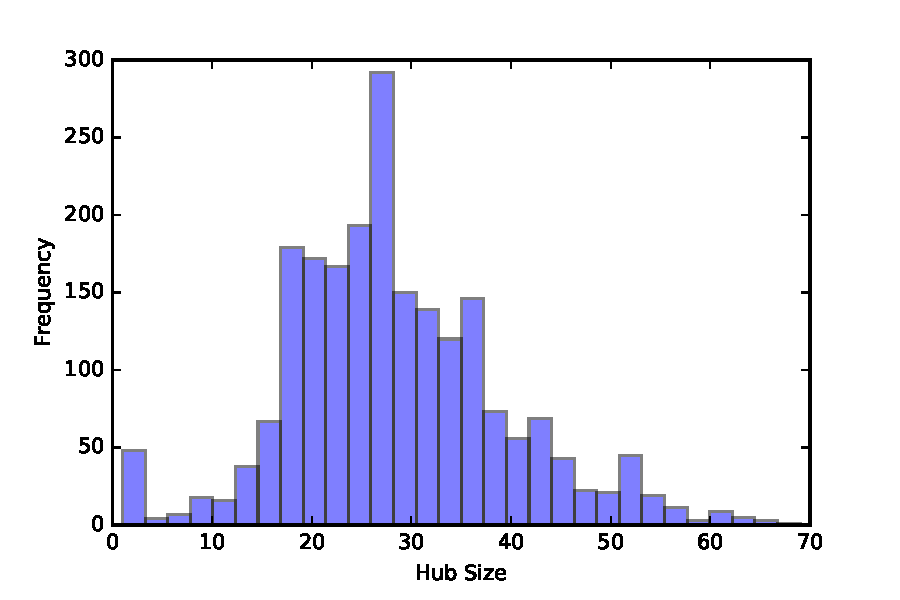
\includegraphics[scale=0.5]{TexImg/SF_bwd_hub_size.pdf}
\end{center}
\end{figure}

\begin{figure} \caption{Histogram frontier queries, Dijkstra (left) and HL (right). $B=25$}\label{fig:SF_query}
\begin{center}
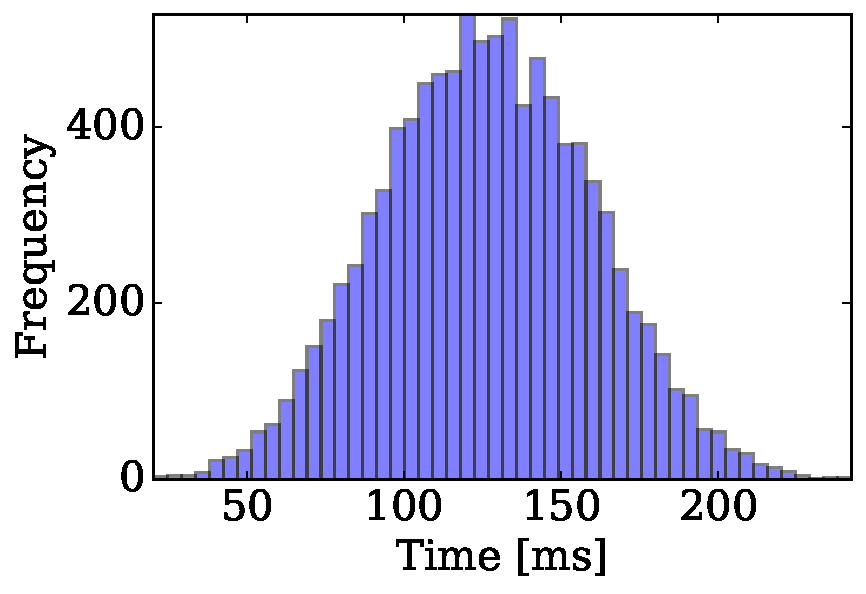
\includegraphics[clip, trim=0.6cm 0.3cm 1.2cm 0.8cm,scale=0.3]{TexImg/SF_query_dij_B25.pdf}
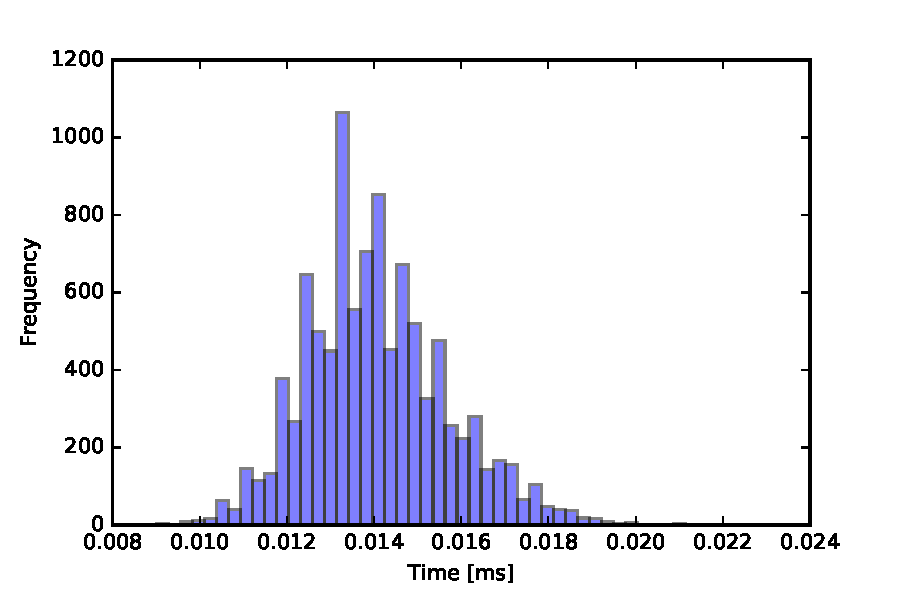
\includegraphics[clip, trim=0.9cm 0.3cm 1.1cm 0.8cm,scale=0.3]{TexImg/SF_query_hl_B25.pdf}
\end{center}
\end{figure}



\begin{figure} \caption{Map of backward size, $B=25$}\label{fig:SF_hub_size_map}
\begin{center}
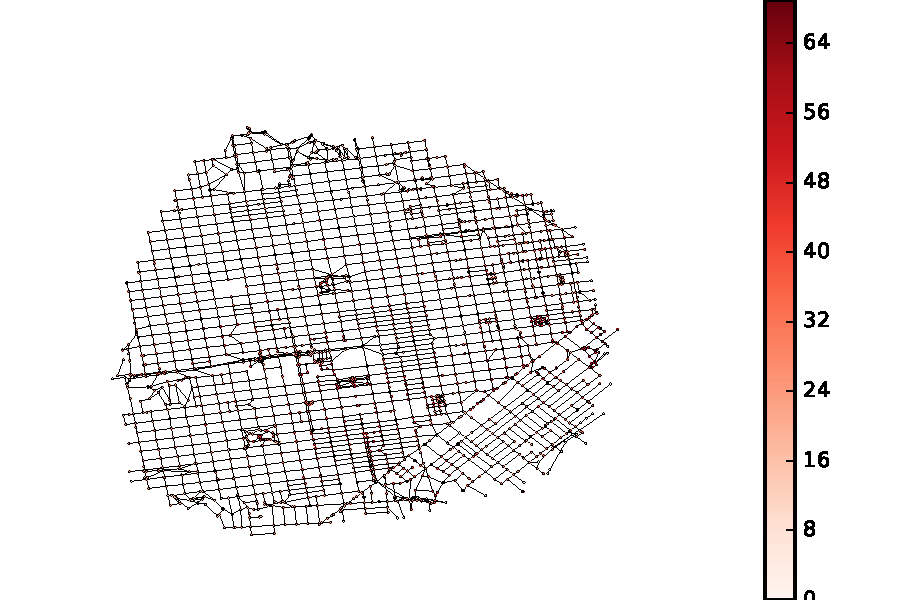
\includegraphics[clip, trim=2cm 1cm 5cm 2cm,scale=0.8]{TexImg/SF_hub_sizes.pdf}
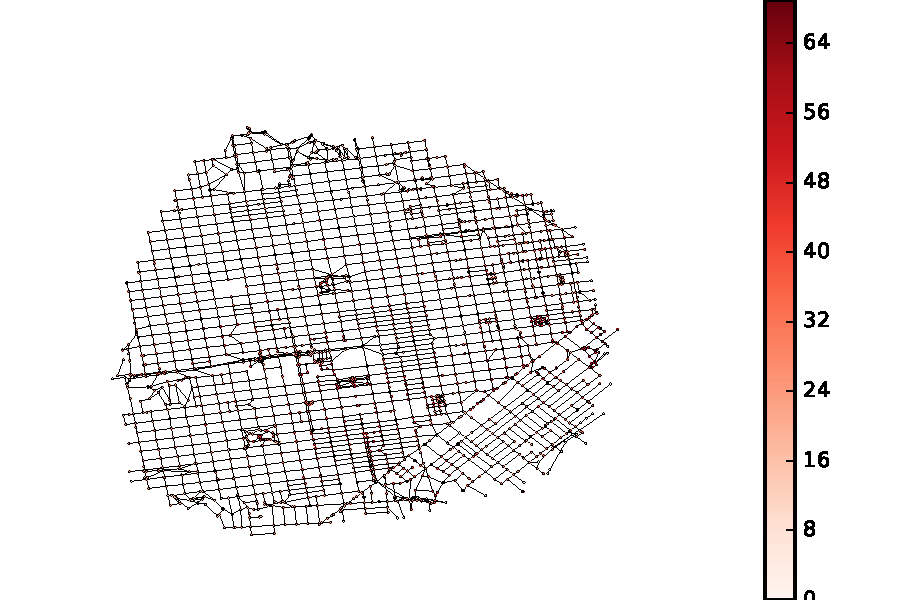
\includegraphics[clip, trim=13cm 0cm 1.1cm 0cm,scale=0.55]{TexImg/SF_hub_sizes.pdf}
\end{center}
\end{figure}